% This is samplepaper.tex, a sample chapter demonstrating the
% LLNCS macro package for Springer Computer Science proceedings;
% Version 2.20 of 2017/10/04
%
\documentclass[runningheads]{llncs}
%
\usepackage{graphicx}
% Used for displaying a sample figure. If possible, figure files should
% be included in EPS format.
%
% If you use the hyperref package, please uncomment the following line
% to display URLs in blue roman font according to Springer's eBook style:
% \renewcommand\UrlFont{\color{blue}\rmfamily}

\begin{document}
%
\title{Contribution Title\thanks{Supported by organization x.}}
%
%\titlerunning{Abbreviated paper title}
% If the paper title is too long for the running head, you can set
% an abbreviated paper title here
%
\author{%
Avinash Kori\inst{1,2}\orcidID{} %
\and Shashank Bansal\inst{2}\orcidID{} %
\and Oscar Estaban \inst{2}\orcidID{}%
\and Joe Wexlar \inst{2}\orcidID{}%
\and Russell Poldrack\inst{2}\orcidID{}}
%
\authorrunning{A. Kori et al.}
% First names are abbreviated in the running head.
% If there are more than two authors, 'et al.' is used.
%
\institute{%
Indian Institute of Technology (IIT), Madras, India
\email{lncs@springer.com}\\
\and Dept. of Psychology, Stanford University, Stanford, USA}
%
\maketitle              % typeset the header of the contribution
%
\begin{abstract}

\keywords{}
\end{abstract}
%
\section{Introduction}


\newpage
\section{Materials and Methods}

\subsection{Overview}
\begin{figure}
 \centering
 \label{fig:overview}
 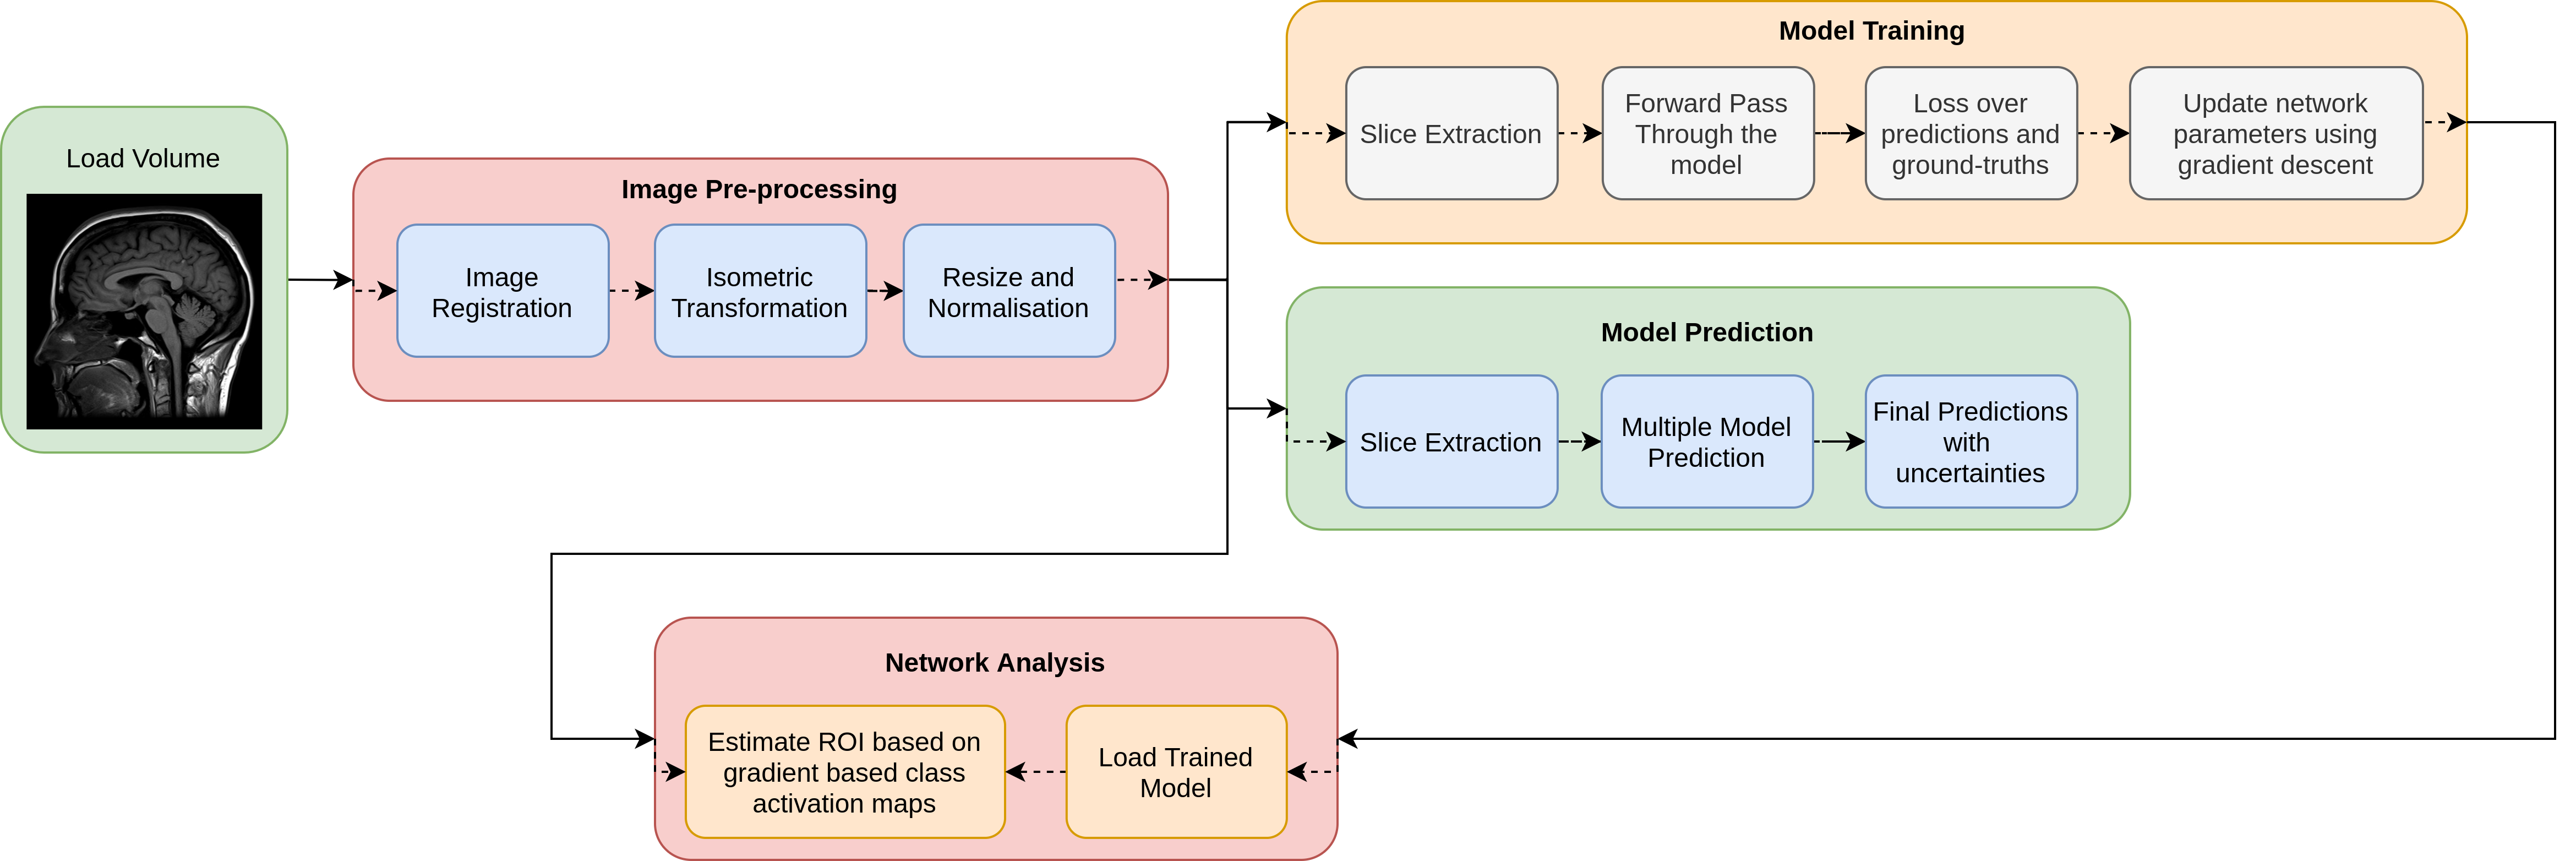
\includegraphics[width=1\textwidth]{images/overview.png}
\end{figure}

The Figure \ref{fig:overview}, describes the overall structure of our framework. The proposed framework detects if the given T1 weighted MR image is faced or defaced. Which in the process involves volume registration to a fixed atlas image, isotropic transformation to standardize the voxel size along all the axis, volume normalization to bound the range of input, followed by slice sampling, and prediction. We perform network analysis to qualitatively quantify the learning of the network using Gradient based class activation maps, and also estimate uncertainities on prediction to provide confidence bounds on the prediction. 

\subsection{Data}
In this task we made use of vaarious openneuro datasets \cite{}. The classification groundtruths wer manually obtained \textbf{process discription}  

In total 1236 volumes with 400 faced and rest defaced. The dataset was split into 3 sets to perform cross validation study. 
\subsubsection{Cross Validation split}

\subsection{Pre-processing of Data}
In terms of preprocessing of the data, volume registration, normalization, resizing, was performed.

\subsubsection{Volume Co-registration}
\subsubsection{Augmentations}
\subsubsection{Resizing and Re-normalization of Volume}
\subsubsection{Slice Extraction}
\subsubsection{Network Architecture}
\subsubsection{Loss function}

\subsection{Training Pipeline}
\subsection{Inference Pipeline}

\subsection{Network Analysis}
\subsubsection{Uncertainty Estimation}
\subsubsection{GradCAM Analysis}


\newpage
\section{Results and Discussion}


\end{document}
